\documentclass[12pt,a4paper]{article}
%\documentclass[8pt]{beamer}
%\usetheme{default}
%\usepackage[font=small,format=plain,labelfont=bf,up,textfont=it,up]{caption}
%\usepackage{setspace}
\usepackage{graphicx}
\usepackage{epstopdf}
\usepackage{natbib}
\bibpunct{(}{)}{;}{a}{}{,}
\usepackage[brazil]{babel}
\usepackage[utf8]{inputenc}
\usepackage {enumerate}
\usepackage{latexsym}
\usepackage{amsmath}
%\usepackage[T1]{fontenc}
%\usepackage{fetamont}
%\usepackage[num]{abntcite}
\usepackage{ mathrsfs }
\usepackage{subfigure}
\usepackage{helvet}
\renewcommand{\familydefault}{\sfdefault}

\newcommand{\farcm}{\mbox{\ensuremath{.\mkern-4mu^\prime}}}%
\newcommand{\farcs}{\mbox{\ensuremath{.\!\!^{\prime\prime}}}}
\newcommand{\ii }{\'{\i}}
\newcommand{\cc }{\c c}
\newcommand{\cca}{\c ca }
\newcommand{\ao}{\~ao }
\newcommand{\cao}{\c c\~ao }
\newcommand{\oes}{\~oes }
\newcommand{\coes}{\c c\~oes }
\newcommand{\eq}{\begin{equation}}
\newcommand{\feq}{\end{equation}}
\newcommand{\dm}{\begin{displaymath}}
\newcommand{\fdm}{\end{displaymath}}
\newcommand{\eqn}{\begin{eqnarray}}
\newcommand{\feqn}{\end{eqnarray}}
\newcommand{\grau}{^{\circ}}
\newcommand{\ba}{\arrowvert_{t_1}^{t_2}}
\newcommand{\bc}{\arrowvert_{0^{\circ} {\rm C}}^{t_2}}
\newcommand{\bb}{\arrowvert_{0^{\circ} {\rm C}}^{t_1}}
\newcommand{\Ms}{$\mathrm{M}_{\odot}$}
%\renewcommand{\labelitemiv}{$-$}
\usepackage{amssymb}
\newcommand{\reg}[1]{#1$^{\tiny{\circledR}}$}
\usepackage[hmargin=2cm,vmargin=2.5cm,bmargin=2cm]{geometry}
\renewcommand{\baselinestretch}{1.2}
%\topmargin -1.5cm
%\leftmargin -2cm
%\rightmargin -2cm
%\oddsidemargin -0.7cm
%\textwidth 16cm
%\textheight 24cm
%\hoffset -1cm 

\usepackage{epic}
\usepackage{arydshln}
\providecommand{\sin}{} \renewcommand{\sin}{\hspace{2pt}\mathrm{sen}}
\numberwithin{equation}{section}

\begin{document}

% CAPA

\thispagestyle{empty}

  \begin{figure}[!htb]
    \centering
    
\includegraphics[scale=0.2]{ufmg.jpg}
    \label{figRotulo}
  \end{figure}

\vspace{3 mm}
\begin{center}
{ESCOLA DE ENGENHARIA}\\
{PROGRAMA DE PÓS-GRADUAÇÃO EM ENGENHARIA ELÉTRICA}\\
\end{center}

\vspace{15mm}
\begin{center}
Luiz Alberto Queiroz Cordovil Júnior \\
Rodrigo Farias Araújo
\end{center}

\vspace{50 mm}
\begin{center}
\textbf{Exercício Computacional 2}\\
\end{center}

\vspace{30 mm}

\vspace{60mm}
\begin{center}
Belo Horizonte - MG\\
Setembro - 2017
\end{center}
\thispagestyle{empty}
\newpage

%CONTRA-CAPA

\thispagestyle{empty}

\vspace{3 mm}
\begin{center}
Luiz Alberto Queiroz Cordovil Júnior \\
Rodrigo Farias Araújo
\end{center}


\vspace{45 mm}
\begin{center}
\textbf{Effect of Rule Weights in Fuzzy Rule-Based \\
Classification Systems}\\
\end{center}

\vspace{25 mm}

\vspace{35mm}
\hspace{9cm}\begin{minipage}[r]{0.45\linewidth}
Trabalho apresentado como parte das exigências para obtenção de nota parcial junto à disciplina Sistemas Nebulosos do PPGEE-UFMG, no S2/2017.\\ 
\\
Prof. Dr. André Paim Lemos
\end{minipage}

\vspace{60mm}
\begin{center}
Belo Horizonte - MG\\
Setembro - 2017

\end{center}

\thispagestyle{empty}
\newpage
\tableofcontents
\newpage

\abstract
Este trabalho apresenta a reprodução da metodologia e dos procedimentos experimentais realizados no artigo de Hisao Ishibuchi e Tomoharu Nakashima (2001), denominado \textit{Effect of Rule Weights in Fuzzy Rule-Baes Classification Systems}, em que são avaliados os efeitos de ponderação de regras em sistemas de classificação fuzzy. A metodologia considera que os valores linguísticos antecedentes de cada classe tem uma única classe consequente, a partir da observação de grau de compatibilidade e de certeza, quando da classificação de padrões. Os autores reivindicam que sistemas de classificação fuzzy com alta performance podem ser projetados sem modificar as funções de pertinência de valores linguísticos antecedentes, quando do uso de ponderação de regras com graus de certeza.
\newpage

\section{Introdução}


De maneira geral os problemas de classificação são aproximações baseadas em dados  no sentido de mapear classes de um conjunto de variáveis. Em sistemas baseados em regras fuzzy, a identificação de padrões e consequente classificação a partir de um número finito (\textit{n}) de atributos é definido como:

\begin{equation} \label{eq1}
Regra~R_{j}:~Se~x_{1}~ \text{é }A_{j1}~e... e~x_{n}~\text{é }A_{jn}~\text{então } Classe~C_{j},~j=1,2,...,N
\end{equation}
em que:
\begin{itemize}
\item $x={x_{1},...,x_{n}}$: $n-$dimensional vetor de padrões;
\item $A_{ij}$: valor linguístico antecedente, $~(i=1,2,...,n)$;
\item $C_{j}$: classe consequente;
\item $N$: número de regras fuzzy SE-ENTÃO.
\end{itemize}

Na abordagem do artigo a ponderação das regras SE-ENTÃO com certos graus de certeza é dada por:

\begin{equation} \label{eq2}
Regra~R_{j}:~Se~x_{i}~\text{é } A_{j1}~e...e~x_{n} \text{é } A_{jn}~\text{então }Classe~C_{j}~com~CF_{j}, j=1,2,...,N
\end{equation}
em que:
\begin{itemize} 
\item $CF_{j}$ é o grau de certeza de cada regra fuzzy SE-ENTÃO $R_{j}$, e, usualmente é um número real no intervalo [0,1].
\end{itemize}

Para esta aplicação foi utilizada a base de dados Iris (1936), do biólogo e estatístico britânico Ronald Fisher, para três espécies da flor \textit{Iris} (\textit{50 setosa, 50 virginica, 50 versicolor}). Considera-se o conjunto de dados separáveis pela discriminação das seguintes características:

\begin{itemize}
\item comprimento e largura da sépala;
\item comprimento e largura da pétala.
\end{itemize}

(Rodrigo, acho interessante plotar aqui gscatter dos dados).

\section{Metodologia}

O método implementado consiste de uma abordagem de seleção de apenas uma classe, ou classe vencedora, durante a fase de classificação, além de, quando na observação da área de decisão haver fronteiras de classificação tendo em vista as regras fuzzy. Ao ponderar-se estas pelo grau de certeza $C_{j}$:

\begin{equation} \label{eq3}
\sum_{p\in Class~C_{j}} \mu_{j}(x_p)=\max(\sum_{p\in Class~k}\mu(x_{p}):k=1,2,...,c)
\end{equation}
em que:

$x_{p}$: número de padrões;

$c$: número de classes.

Como pode ser visto na equação (\ref{eq3}) a classe consequente $C_{j}$ é especificada como a classe dominante no espaço fuzzy correspondente ao antecedente de cada regra fuzzy SE-ENTÃO. Aplicando-se a definição demonstrada na equação (\ref{eq2}), um novo padrão $x{p}=(x_{p1},...,x_{pn}))$, pode ser definido como:

\begin{equation} \label{eq4}
\mu_{j}^{ *}(x_{p}).CF_{j}=\max\lbrace\mu_{j}(x_{p}).CF_{j}:~j=1,2,...,N\rbrace
\end{equation}

A classe consequente pode ser determinada a partir de padrões de treinamento, como também se esta é a dominante em determinado subespaço do espaço fuzzy. Como toda regra tem sua própria área de decisão, cujo tamanho é determinado pelo grau de certeza e pelo antecedente linguístico das funções de pertinência, a abordagem realiza mudança na dimensão da área de decisão por ponderação. Neste sentido o grau de certeza é dado por:

\begin{equation} \label{eq5}
CF_{j}=\frac{\beta_{Classe~C_{j}}(R_{j})-\overline{\beta}}{\sum_{k=1}^{c}\beta_{Classe~k}(R_{j})}
\end{equation}
em que $C_{j}$ é a classe consequente e:

\begin{equation} \label{eq6}
\overline{\beta}=\frac{\sum_{k\neq C_{j}}\beta_{Classe~k}(R_{j})}{(c-1)}
\end{equation}

As formulações indicadas nas equações (\ref{eq5}) e (\ref{eq6})  estendem a determinação do grau de certeza para um problema de classificação com $c$ classes.

\subsection{Procedimentos Computacionais} \label{PC}

Inicialmente o modelo foi descrito como sendo função das duas primeiras variáveis do conjunto de dados, os quais correspondem ao comprimento e largura da sépala de todas as classes.

Em termos de modelagem... (Acho que seri abom exemplificar as funções de pertinência que foram utilizadas).

\subsection{Regiões de Classificação}

Nesta etapa, a partir da definição do grau de certeza na observação das características do conjunto de dados, o sistema de classificação converge para uma discriminação das classes (espécies), como uma área de decisão, a partir da especificção de cada regra e da fronteira de classificação.

Conforme indicado na seção \ref{PC}, como função de duas variáveis, a área de decisão, com a utilização de t-norma do produto é indicada na Figura \ref{tnp}:

\begin{figure}[ht] \label{tnp}
\centering
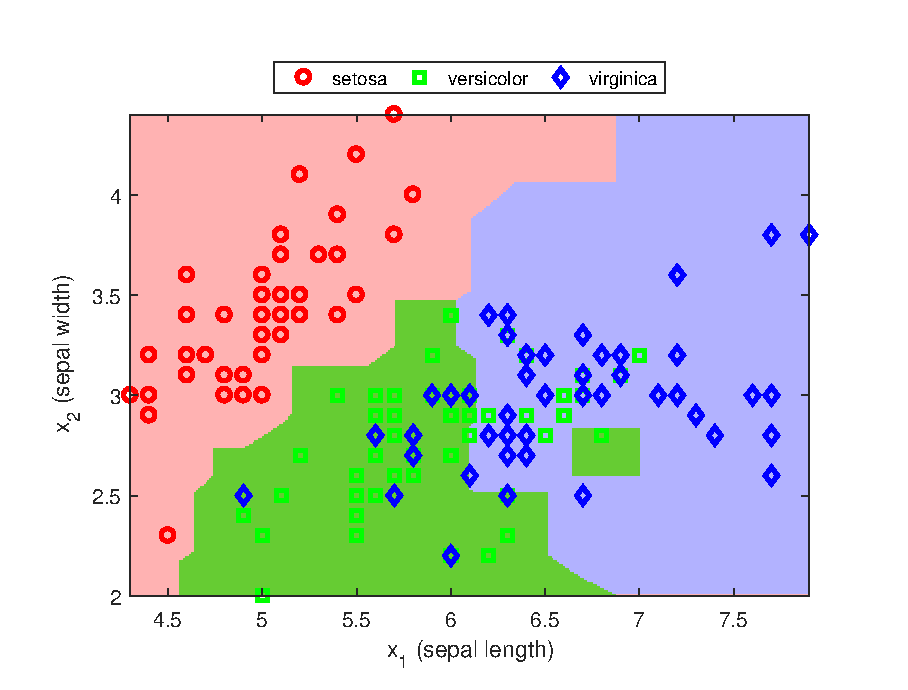
\includegraphics[width=0.7\textwidth]{product.eps}
\caption{Área de decisão usando a t-norma produto.}
\label{fig:product}
\end{figure}

Com a utilização da t-norma mínima:

\begin{figure}[ht] \label{tnm}
\centering
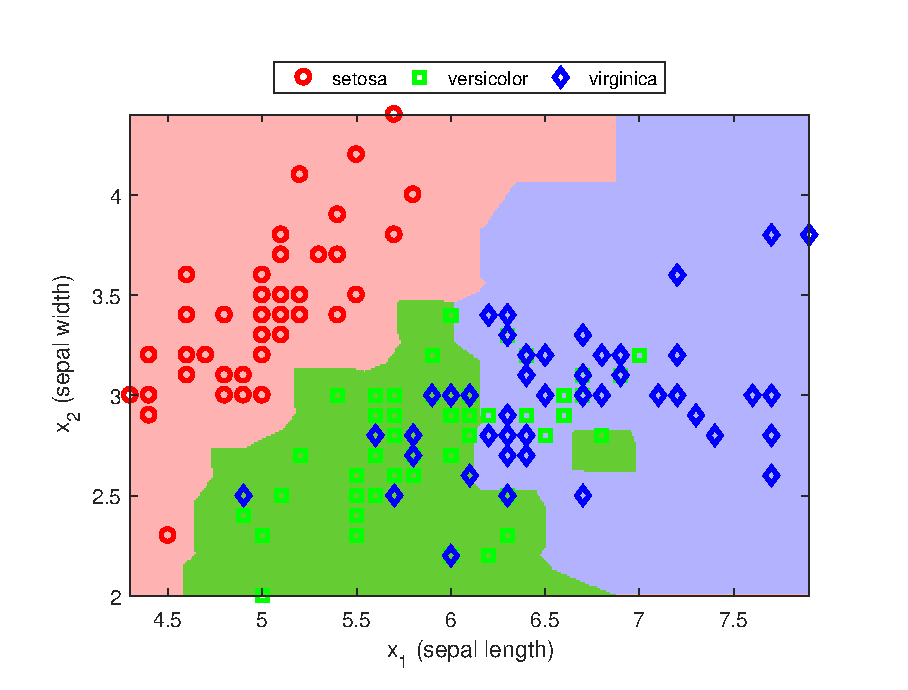
\includegraphics[width=0.7\textwidth]{minimum.eps}
\caption{Área de decisão usando a t-norma mínimo.}
\label{fig:minimum}
\end{figure}

O particionamento do espaço de entrada (variáveis) fornece o suporte para formulação de regras que estejam relacionadas a este subespaço.

Em termos práticos, a utilização destes dois tipos de conjunções lógicas, implica na análise das regras, sejam elas condicionais (relação interna entre antecedentes e consequentes) e incondicionais, de maneira geral afirmativas. 

O que se percebe é que o processo de inferência, ou seja, o processo de avaliação das regras para cada subconjunto fuzzy acaba por estabelecer relações. Para este caso, no sistema de classificação, ao combinar-se o conjunto de dados de entrada, ao menos uma regra deve ser ativada, ponderada pelo grau de certeza.

O operador mínimo da t-norma busca e o operador do produto algébrico, no que se refere a inferência composicional de regras, estabelecem a interseção entre regras para a dedução de uma sequência lógica.



\subsection{Treinamento e Validação}

Na abordagem computacional, por meio da técnica de validação cruzada, cada conjunto de espécies foi separado em subconjuntos de treinamento e teste representados, com dimensão de 70\% e 30\%, respectivamente de cada classe de padrões.

Para todas as classes, no total, quatro dados de entrada aplicados a três espécies, com 50 amostras. Como ferramenta de aprendizagem, os conjuntos de treinamento e teste, foram determinados observando-se os percentuais em 35 e 15 amostras, respectivamente, para cada classe $C_{j}$.

Neste sentido, na etapa de treinamento, a partir de aprendizado supervisionado, houve a classificação inicial das amostras, como função da quantidade de regras e dos graus de certeza, no sentido de se estabelecer as condições e parâmetros iniciais do sistema de classificação.

A partir destes, houve a implementação das características de contexto adquiridas na etapa de treinamento, no sentido de aferir-se a performance do sistema de classificação.

Os experimentos foram realizados N vezes, para 2 até n regras, com o propósito de se observar o limiar de convergência e paridade entre o erro do conjunto de treinamento e erro no conjunto de teste. As amostras foram escolhidas aleatoriamente dentro dos subconjuntos e testadas para cada conjunto de regras, por n repetidas vezes.

(Separar os gráficos Rodrigo).

\begin{figure}[ht]
\centering
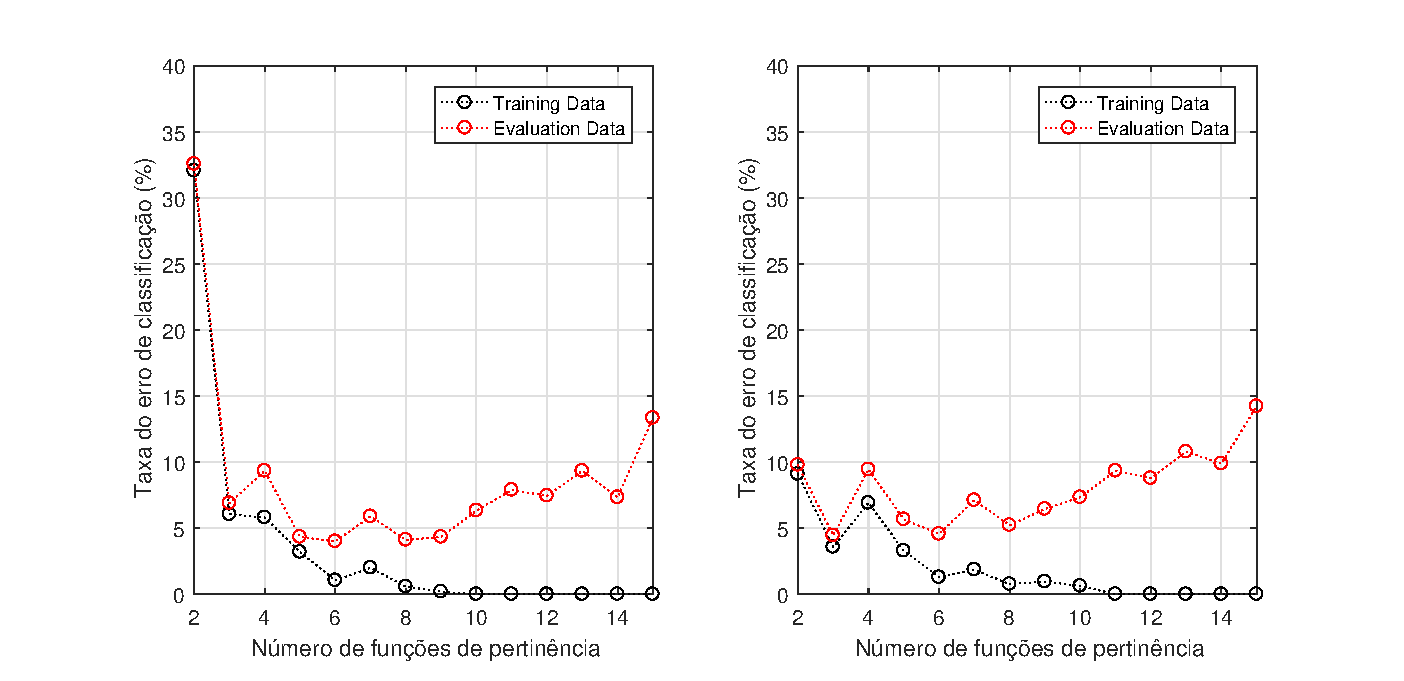
\includegraphics[width=0.7\textwidth]{error.eps}
\caption{Trajetória do erro em relação ao número de funções de pertinência.}
\label{fig:product1}
\end{figure}

\newpage
\section{Conclusões}

A utilização de sistemas de classificação baseados em regra a partir da ponderação por grau de certeza, oferece uma solução baseada em conhecimento dedutivo, o que em termos práticos, implica na sobreposição de uma regra dominante sobre outra no espaço fuzzy, ou seja, na combinação de $n$ regras, pelo menos uma, por inferência composicional, forma a consequência lógica.

Todos os procedimentos realizados no artigo e replicados em simulações compõem base de conhecimento por raciocínio aproximado pelo fato da definição de consequentes a partir de relações de compatibilidade em função dos graus de certeza. Neste sentido as conclusões das conjunções lógicas, seja pelo operador mínimo ou de produto da t-norma, são baseadas no domínio de uma regra sobre a outra no espaço de decisão, sendo este ponderado pelo grau de certeza..
\newpage

\section*{Referências}
\addcontentsline{toc}{section}{\protect\numberline{}Referências}%

[1] ISHIBUCHI, Hisao; NAKASHIMA, Tomoharu. Effect of rule weights in fuzzy rule-based classification systems. IEEE Transactions on Fuzzy Systems, v. 9, n. 4, p. 506-515, 2001.

\end{document}
